\documentclass{article}
\usepackage{listings}
\usepackage{amsmath}
\usepackage{siunitx}
\usepackage{graphicx}

\title{Stats Week 9}
\author{Rvail Naveed: 17321983}

\begin{document}
    \maketitle
     

    \section*{Q1(a)}
        Code for gradient descent included in zip.

    \section*{Q1(b)}
        \subsection{$\alpha = 1$}
            The gradient descent algorithm becomes unstable because the learning rate parameter 
            is too high, causing it to jump between 0.5 and -0.5 constantly. It is not able to come 
            up with an answer in a reasonable timeframe.
    \pagebreak

        \subsection{$\alpha = 0.1$}
            The algorithm is able to find the minimum in 32 steps, an adequate amount of time.
            \begin{itemize}
                \item Steps taken: 32
                \item Minimum occurs at: 0.00
            \end{itemize}
            \begin{figure}[h]
                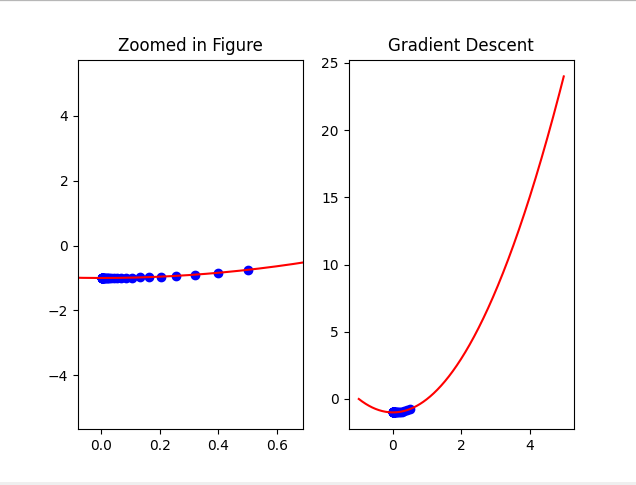
\includegraphics[scale=0.5]{a.png}
                \caption{$\alpha = 0.1, x_start = 0.5, precision = 0.0001$}
            \end{figure}

    \pagebreak

        \subsection{$\alpha = 0.01$}
            The learning rate is too low, so it takes many more steps to find the minimum. In reality
            the minimum was probably found before the completion of all steps but the learning rate being too low
            prevented it from stopping earlier.
            \begin{itemize}
                \item Steps taken: 229
                \item Minimum occurs at: 0.00
            \end{itemize}
            \begin{figure}[h]
                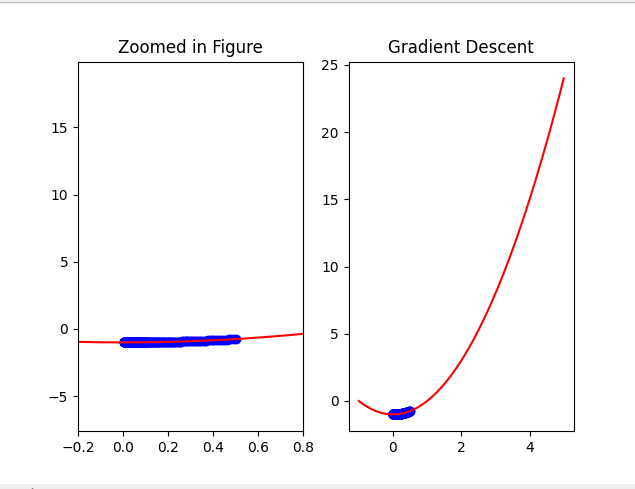
\includegraphics[scale=0.5]{b.png}
                \caption{$\alpha = 0.01, x_start = 0.5, precision = 0.0001$}
            \end{figure}           

    \pagebreak

    \section*{Q1(c)}
        Code for random strategy included in zip. \break
        *Only plotted the x values for which $f(x_{k+1}) < f(x)$

        \begin{itemize}
            \item Minimum: 0.00
            \item Steps: Varies between 5000-50,000
        \end{itemize}

        \begin{figure}[h]
            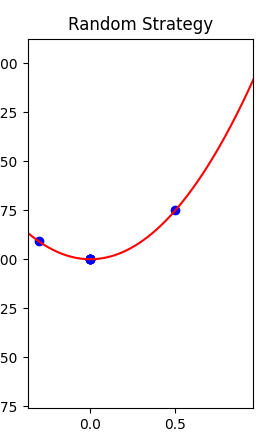
\includegraphics[scale=0.5]{c.png}
        \end{figure}    
    
        \section*{Q1(d)}
            Took many more steps to find a suitable x value in the vicinity
            of the current x. Since picking the x point is random, results vary drastically.
            This is in stark contrast to gradient descent which is very easy to control via the 
            learning rate.

        \section*{Q2(a)}
            This can be achieved using the Bag of Words approach described in the slides:

            \begin{itemize}
                \item Delete all the little words, truncate word endings.
                \item Form a list of all the unique words that are left, and number them 1-n.
                \item Map the text of a review to a vector of length n by setting i of the vector equal to the number of times the ith word
                      in the dictionary appears in the review.
                \item Then apply logistic regression methods as usual with this new vector.
                \item Using model: $\frac{P(Y=1 | X=x) = 1}{1 + exp(-z)}$
            \end{itemize}
        
        \section*{Q2(b)}
            Assumptions:
            \begin{itemize}
                \item There is a linear relationship between the features and target.
                \item X values in the sample are not all the same (Variability in X values is positive)
            \end{itemize}
        
        \section*{Q2(c)}
            \begin{itemize}
                \item Randomly split training data into training set and test set.
                \item Train model on the training data to select parameter values which minimise cost function.
                \item Evaluate accuracy of predictions using test data.
                \item Repeat above steps to obtain a set of prediction errors.
                \item Use those to estimate distribution and so the confidence interval.
            \end{itemize}
    
\end{document}